\documentclass{sigchi}

\usepackage{amsmath}
\usepackage{amssymb}
\usepackage{amsfonts}
\usepackage{bm}
\usepackage{xcolor}
\usepackage{booktabs}
\usepackage{floatrow}
\usepackage{blindtext}
\usepackage[english]{babel}
\usepackage[utf8x]{inputenc}
\usepackage[colorinlistoftodos]{todonotes}
\usepackage{graphicx}
\usepackage{tabularx}

% \long\def\/*#1*/{}

% https://www.overleaf.com/5725947pwvcgh#/18690373/

%Achievement, Relationship, and Engagement (ARE): Using 
% 
\title{Deep Reinforcement Learning for Modeling User Strategies and Motivations from Massive Game Behavioral Data}

\numberofauthors{4}
\author{%
  \alignauthor{Leave Authors Anonymous\\
    \affaddr{for Submission}\\
    \affaddr{City, Country}\\
    \email{e-mail address}}\\
  \alignauthor{Leave Authors Anonymous\\
    \affaddr{for Submission}\\
    \affaddr{City, Country}\\
    \email{e-mail address}}\\
  \alignauthor{Leave Authors Anonymous\\
    \affaddr{for Submission}\\
    \affaddr{City, Country}\\
    \email{e-mail address}}\\
  \alignauthor{Leave Authors Anonymous\\
    \affaddr{for Submission}\\
    \affaddr{City, Country}\\
    \email{e-mail address}}\\
}


\begin{document}
\maketitle

\abstract

Massively multiplayer online role-playing game (MMORPG), such as World of Warcraft (WoW), attracts millions of users and many of them spend thousands of hours playing games online. 
Understanding their behaviors and the underlying motivations is of great interests to game designers and researchers, and also to parents and educators. 
We employ deep reinforcement learning algorithm to model users' playing strategies, and propose an inverse reinforcement learning algorithm to model their motivations. 
We use a massive and complex online game behavioral dataset, World of Warcraft Avatar History (WoWAH), which records over 70,000 users' log data spanning 3 years time period. 
Our trained model not only can predict users' behaviors with a high level of accuracy. 
Moreover, it can also reveal users' motivation dynamics in terms of \textit{achievement}, \textit{social}, and \textit{immersion}. 

\category{H.5.m}{Information Interfaces and Presentation (e.g. HCI)}{Miscellaneous} \category{I.2.1}{Artificial Intelligence}{Applications and Expert Systems}
\keywords{Online game motivation; game design; reinforcement learning; apprenticeship learning;}

\section{Introduction}

Understanding Massively multiplayer online role-playing game (MMORPG) games satisfaction mechanism and user behaviors could be non-trivial. 
As human players have a mixed feeling from different perceptions and they act not for a concrete, explicit objective such as winning an episode or taking high scores. 
While it's plausible to build a gaming bot from the player log data, to advance in the game, it ignores other dimensions of motivation which the players also care about. 
The game designers and researchers, also parents and educators, are, however, keen to reveal the underlying mechanism instead of just mastering the game.

\begin{table}[t]
    \centering
    \caption{WoWAH Dataset Attributes}
    \begin{tabularx}{\textwidth}{lX}
        Attribute & Value \\
        \midrule
        Duration & 1107 days \\
        Sample Interval & Every 10 minutes \\
        \#Users & 70,000+ \\
        Locations & One of 165 zones
        \label{tbl:wowah}
    \end{tabularx}
\end{table}

Take World of Warcraft (WoW), which is one of the most successful MMO games in the world, as an example. 
It's massive, and multiplayer as millions of players pay to subscribe the game platform. 
On the platform players can communicate with others, finish some quests cooperatively, compete with each other, and even build their own guilds. 
WoW also provides different kinds of races, careers and optional requests that could serve players extra flexibility to evolve different game styles. 
With all those features the players' behavior can be very complex, as they receive different dimensions of satisfaction which eventually compose the general reward system of the game.
%With all those features the players receive many different dimensions of satisfaction which eventually compose the general reward system of the game.
%It was released by Blizzard in 2004 and stills continuing updating nowadays.

For its huge research and commercial value to study game players' behavior, attentions has been drawn for both qualitative and quantitative studies.
In contrary to WoW, many studies are conducted on single-player game or multi-player but zero-sum game. 
For those environments, advancing usually serves as the sole criterion of game motivation.
In Game Trace Archive (GTA) \cite{guo2012game} who has been collecting online gaming data since 2012, 10 out of 14 traces are from the game environment stated above.
Although reinforcement learning (RL) algorithms have been succeeded in mastering such kind of games, it does not help figuring out the underlying motivation, neither the complex reward mechanism existing in MMO games and in real world. 
Even for those studies in WoW, datasets such as Very Large WoW Armory Dataset \cite{Bell2013a} focus on certain campaigns instead of general gaming strategies because of its short time span and fine-grained actions (such as spelling).
Taking that into consideration, the episodes recorded is still mostly about advancing, and game tactics.

World of Warcraft Avatar History (WoWAH) dataset \cite{lee2011world}, published in 2011, records the location (in term of zone) of over 70,000 users every 10 minutes, together with some essential statistical analysis. 
%\footnote{we talk about the reason choosing this dataset in the first section of \textit{Method}} 
However, those analysis and the further studies based on the dataset are far from fully utilization of the data. 
While some of them use simple classifiers or clustering for behavior analysis \cite{suznjevic2011mmorpg,drachen2014comparison}, others focus on forecasting future events such as unsubscribing of game or violation of terms \cite{bauckhage2015clustering,thawonmas2011analysis,lou2012forecasting}. 
Few of them are effectively modeling the interaction between the players and the game environment, neither on another dataset. 
On the other hand some studies tries to conduct studies on player motivations \cite{Bell2013a}, but only able to apply some basic machine learning tools such as clustering.  
%First, statistical approaches usually collapse the data over the time scale, which ignores the dynamic of both gaming environment and players.

We re-employ the WoWAH dataset in a totally different way: to model human-computer interaction (HCI) from a reinforcement learning perspective. 
The human player and computer are characterized by a pair of agent and environment, as shown in Fig. \ref{fig:chi}. 
We show an interesting analogy between the traditional user experience model on the left, and the reinforcement learning scheme on the right. 
In the model, each player is modeled by an agent, whose zone transactions are regarded as the actions of the agent. 
Instead of manually collect opinions from the players as the feedback, we utilize the actual reward system of the game which provide diverse satisfactions.
A common difficulty in WoW and most of the cases in HCI is that the definition of reward is implicit or partial, e.g. we can't tell if a play is optimal simply by looking at the experience gain credited to this play. 
Even if some could try building a reward function according to their knowledge of certain environments, it worth to note that figuring out the reward mechanism itself is a valuable task. 
In fact, the, usually underlying, reward mechanism gives the most succinct description of the task. 
Especially for the developers of the environment, it's a way to give a quantitative representation of what they have designed.
%Existing models in reinforcement learning succeed in modeling human behaviors by training the agent to maximize the explicitly defined reward.

\begin{figure}[t]
    \centering
    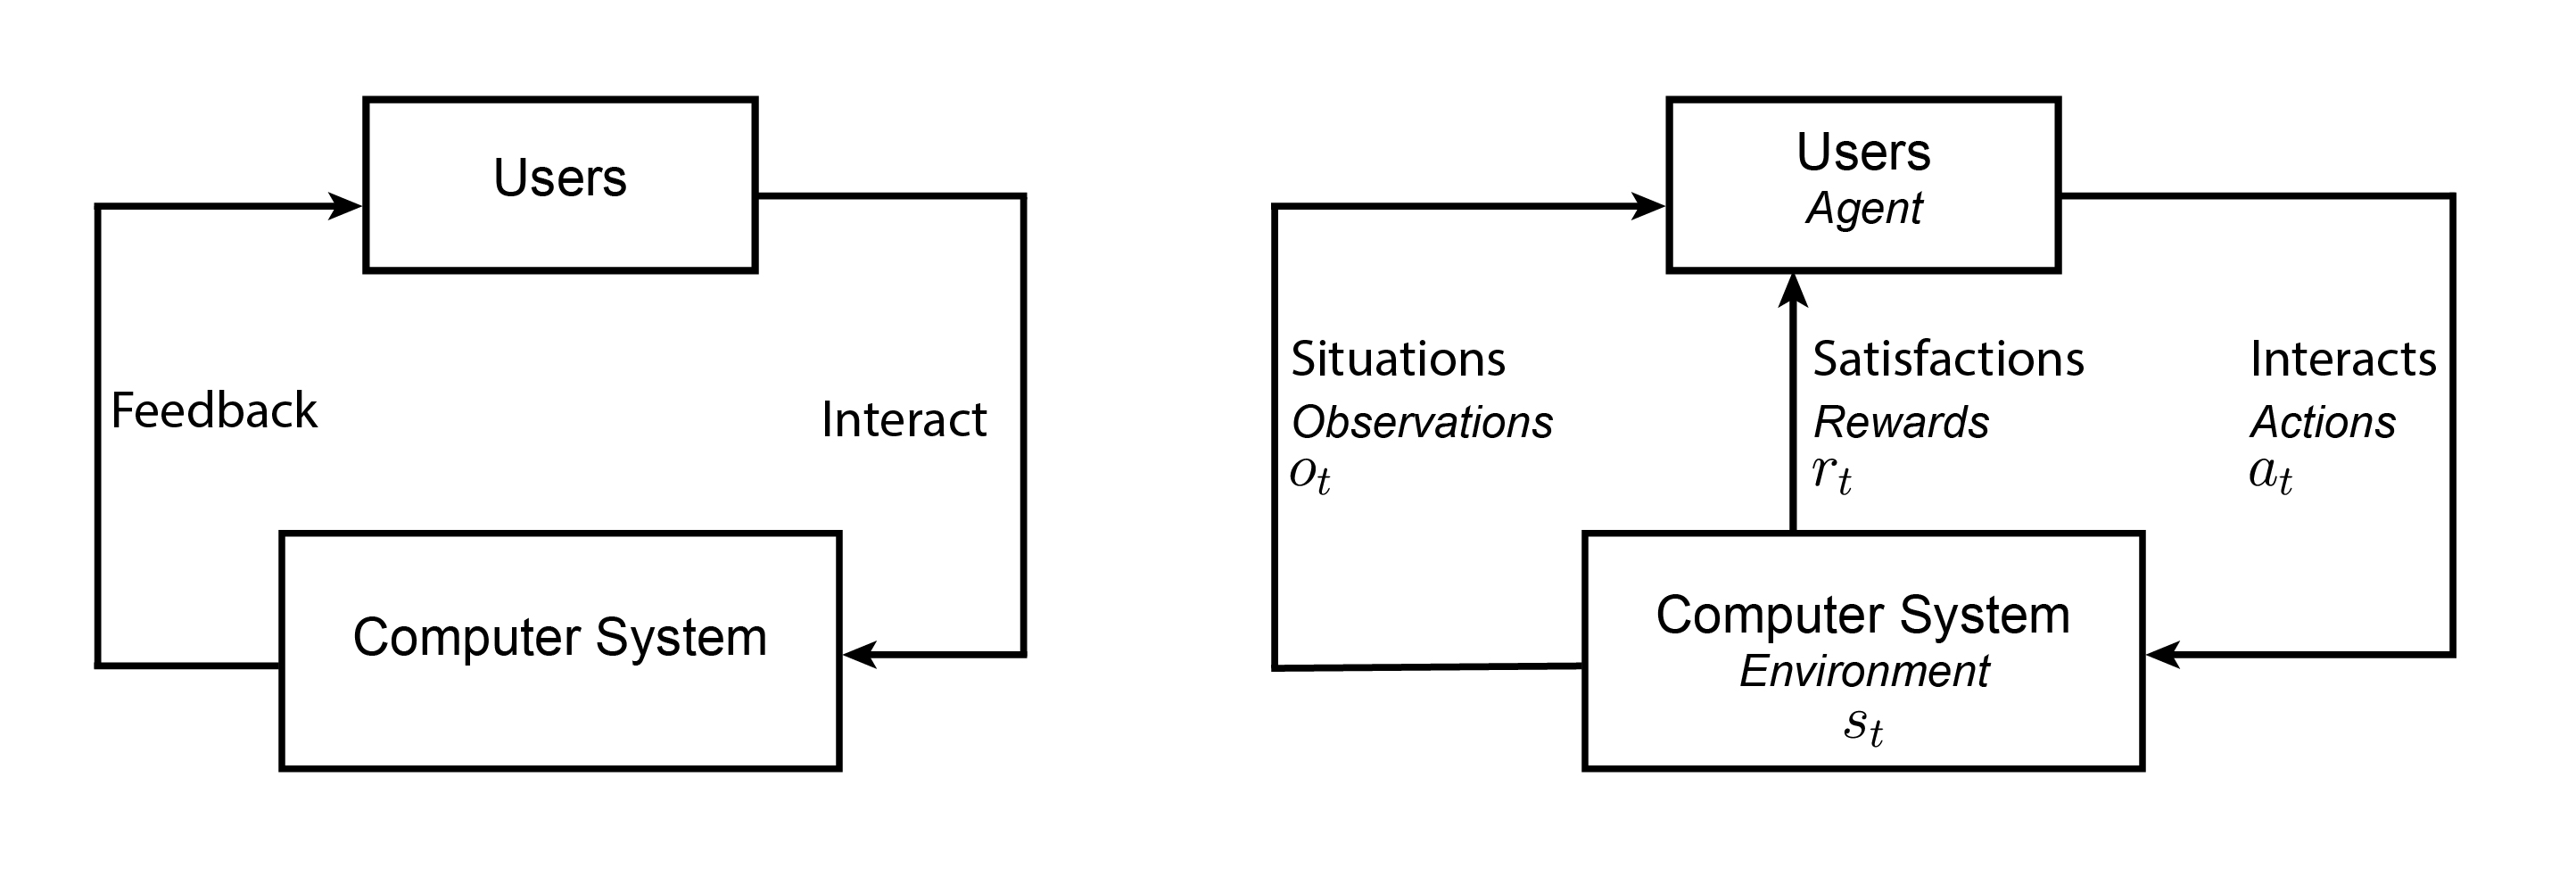
\includegraphics[width=\textwidth]{figs/rl-vs-chi.jpg}
    \caption{User experience model (left) and reinforcement learning model (right)}
    \label{fig:chi}
\end{figure}

The process of recovering the reward function is inverse reinforcement learning (IRL). 
In a data-driven manner, it recovers the underlying reward function which induces the recorded user behaviors, simply by assuming that those players are trying to maximize their rewards. 
Most of the IRL algorithms require we have access the dynamic of the environment, that is in WoW, we simulate the player's action and observe the feedback from the environment. 
Although we obviously don't have it, we address it by proposing an IRL algorithm based on purely off-policy learning. 
The model analyzes the behaviors of the players, using the trajectories composed of player locations, and returns the reward function under which those trajectories are most plausible to happen. 
With the recovered reward, we train an agent to best mimic the general user behavior in WoWAH dataset. 
As our reward recovery algorithm works for any set of trajectories, we conduct future studies to character the dynamics of the game environment thus how design factors working on user behaviors, and compare different groups of users to examine the divergence of game motivations.
Consistency was observed between our model results and empirical analysis on the game environment. 


\section{Related Work}

\subsection{Online Game Player Motivation And Rewards}

One reason that online games appeal so many players is that it provides the possibility for different kinds of play styles. 
The same online game may have respective meanings for different players. 
In the game environment, players pursue certain kinds of satisfactions they want by conducting their actions, which eventually compose the user behaviors we observe. 
Hence, it's natural to assume a user's behaviors are highly correlated with the user's specific reward mechanism, represented by their demanding satisfactions. 
And for game designers and research, finding the demanding satisfactions of users could yield better understanding of the game, and ease to serve the users with better experience. 

Previous study categories the satisfactions into three major aspects, namely, achievement satisfactions, social satisfactions, and immersion satisfactions \cite{yee2006motivations}. 
It was then divided into ten subcategories, briefed in Table. \ref{tbl:components}. 
More details are provided in the original paper and the author's another paper about MMORPG motivation \cite{yee2006demographics}. 
The satisfaction model is popular in online game researches, and provide some basic understand of the online game motivation.
However, the weights associated with these ten kinds of satisfactions are still unknown. 
As the weights basically depicts a user's profile, it would be very meaningful if they can be recovered in a purely data-driven process, i.e. based on the user's playing history.

\begin{table}
\caption{Components of game motivation}
\begin{tabularx}{\textwidth}{lX}
    Components & Sub-components \\
    \midrule
    Achievement & Advancement, Mechanics, Competition \\
    Social & Socializing, Relationship, Teamwork \\
    Immersion & Discovery, Role Playing, Customization, Escapism
    \label{tbl:components}
\end{tabularx}
\end{table}

\subsection{Player Behavior Analysis in Online Games}



\subsection{Reinforcement Learning and Inverse Reinforcement learning}

Reinforcement learning (RL), especially deep reinforcement learning (DRL), is an emerging domain inspired by behaviorist psychology. 
In RL, the agent performs in an online environment and conducts a sequence of actions.
Instead of being taught of the correct policy, the agent get a reward for each of its actions and evolves itself from its own pains and pleasures. 
Interestingly, it deals with the common trade-off between exploration and exploitation, which presents in many real life situations. 
Success in maximizing cumulative reward in the future, rather than exploiting current reward, could lead to expert level game play, which is also a intrinsic property of expert human players.
For example, to level up quickly in a game in a long-term perspective, the player has to conduct some preparation works which does not necessarily benefit its leveling up in the near future.

RL is able to formulate many problems in user behaviors analysis and modeling. 
For example, the recent advances in RL conduct superior play compared with professional human players in the game of Go \cite{silver2016mastering}, Atari 2600 \cite{mnih2015human}, and Poker \cite{heinrich2016deep}. 
It's also employed to model users' clicking and browsing behaviors for online shopping websites, and robotics and optimal controls.  It's worth to note that DRL makes it possible to handle complex environment with high-dimension observation spaces, making it possible to model a wide range of problems such as WoW user behavior analysis.

A great challenge is that the reward scheme of the environment is not explicitly given in most problems in user behavior analysis and modeling. 
For example, the user experience of a software or an online game is the combination of different kinds of satisfaction, processed by the human brains.
In some of those cases, inverse reinforcement learning (IRL) \cite{ratliff2006maximum,ng2000algorithms} recovers the underlying reward function, using the recorded actions of the users.
Further applying apprenticeship learning algorithms \cite{abbeel2004apprenticeship} could mimic the policy that was used to generated the recorded data.
But to invoke those IRL algorithms, it usually requires the access of the dynamic of the environment, which is not doable in online gaming analysis. 
As applying IRL on users' behavior log could help the developers understand the intention of the user, New IRL algorithms are needed to be designed to comply with the problem without the access to the dynamics.

\section{Method}

\subsection{Dataset Description and Reinforcement Learning Formulation}

We use World of Warcraft Avatar History (WoWAH) dataset \cite{lee2011world}, collected from realm \textit{TW-Light's Hope} during 1st Jan 2006 to 10th Jan 2009. 
It contains 70,055 users after we filtering out those with too short playing history, each with 516.21 time intervals (5162.1 minutes) spent online on average.
During each of the 10-minute interval, the user's location, in terms of zone ID (ranging from 1 to 165), was recorded.
The players' trajectories was composed of a sequence of locations, which reflect their playing strategies.
We find datasets with coarse-grain records, i.e. 10-minute interval, most suitable to model user behaviors. 
They are preferred than those with interval of a few seconds, which instead focus on game tactics and user mobility \cite{Bell2013a,shen2014characterization}.
Moreover, the dataset contains many different kinds of users: both novice and expert, guild members and isolated players, low-level and high-level players etc. with their respect class, and race in game. 
The detailed attributes are listed in Table~ref{tbl:wowah}.

In a reinforcement learning perspective, we treat an user as the agent who conduct an action every time interval.
An action here corresponds to a zone transaction or staying in the current zone. 
The user receives current stats of its profile as the observation, after each action it has conducted.
The observation includes all the attributes recorded in the dataset, after a pre-processing to reduce the redundancy.
To make the data consistent, we ignore the time intervals where a user being offline, and concatenate multiple game session of a player to build the trajectory.
As the exact reward mechanism remains unknown, the RL policy can only be learned after the reward function is properly modeled.

We process some preparation for the reward modeling. 
Borrowing the result in game motivation analysis \cite{yee2006motivations}, we define and compute different of satisfactions using the WoWAH dataset.
The constructions of $f_1,\dots, f_5$ are illustrated in Table \ref{tbl:satisfactions}, which are able to be calculated from the observations the user receives.
With those value, we assume the reward function which the agent tries to optimize during the game play, is associated with the five different dimensions of satisfactions. 
We further address the relation between the reward function, and the satisfactions.
Note the value of $f_1,\dots, f_5$ are normalized into the same scale.

\begin{table}
\caption{Different types of satisfactions (Sat.), and their corresponding categories}
%\begin{tabular}{llp{4.8cm}}
\begin{tabularx}{\textwidth}{lX}
    Sat. & \textbf{Category} \& Definition \\
    \midrule
    $f^1$ & \textbf{Advancement} The speed the user collecting experience and leveling up in game. It's the most common satisfaction a user could receive. \\
    $f^2$ & \textbf{Competition} The satisfaction the user get by joining battleground or arena and competing with human opponents. \\
    $f^3$ & \textbf{Relationship} The long-term relationship with the user's guild, which is quantified by the time elapse since the user joining its guild. \\
    $f^4$ & \textbf{Teamwork} The satisfaction the user get by playing in a zone which is featured by teamwork, e.g. \textit{Battleground}, \textit{Arena}, \textit{Dungeon}, \textit{Raid}, or a zone controlled by \textit{The Alliance}. \\
    $f^5$ & \textbf{Escapism} Escapism begins to accumulate if the user has been online for a long session or has been regularly login to the game for many days.
    \label{tbl:satisfactions}
\end{tabularx}
\end{table}

\subsection{Reward Mechanism Modeling}

We introduce our algorithm to recover the underlying reward mechanism of the players, using the trajectory $\tau$ of a user or a group of users. 
Assume the reward a user receives is the convex combination of the five kinds of satisfactions listed in Table. \ref{tbl:satisfactions}. 
Let $f_t=(f_t^1,f_t^2,f_t^3,f_t^4,f_t^5)$ be the vector of satisfactions the user received at time $t$, we have the total reward the user receives at time $t$ 
\begin{equation*}
r_t=\phi^Tf_t,
\end{equation*}
where $\phi$ is the combination weight with $||\phi||_1=1, \; \phi \geq 0$. Assume at each time step, the user tries to take an action $a$ according to the current game state so as to maximize the best expected cumulative discounted (with discount $\gamma$ over time) reward (known as the action-value function) $Q^\ast(s, a)$, where
$$Q^\ast(s,a)=\mathbf{E}[R_t | s_{t}=s, a_{t}=a | \pi^\ast]$$
and
$$R_t=\sum_{t^\prime\geq t}\gamma^{t^\prime-t}r_{t^\prime}=\sum_{t^\prime\geq t}\gamma^{t^\prime-t}\phi^Tf_{t^\prime}.$$
The term $\pi^\ast$ indicates optimal policy, described by a distribution $\mathbb{P}(a|s)$ over the feasible action space $\mathcal{A}(s)$. In this setting, the weight $\phi$ must satisfy that the action the user has taken must induce a larger $Q^\ast$ value than any other valid action would have done. This optimality infers that
\begin{equation}
Q^\ast(s,a) \geq \max_{a^\prime \in A(s)}Q^\ast(s,a^\prime) \label{eqn:irl}
\end{equation}
is satisfied for all $(s,a)$ pairs appeared in the user's trajectory. Consider the existence of possible sub-optimal actions conducted by the user, we introduce slack variables $\xi_{s,a}$ into the problem formulation. Let $\xi_{s,a}$ be the difference of the actual action-value $Q^\ast(s,a)$, and the largest possible action-value $\max_{a^\prime \in A(s)}Q^\ast(s,a^\prime)$ whenever Eq. \eqref{eqn:irl} is not satisfied, and zero otherwise. We minimize the summation of $\xi_{s,a}$ over the recorded user's trajectory
\begin{equation}
-C\sum_{s,a} \left[\min(0, Q^\ast(s,a) - \max_{a^\prime \in A(s)\backslash a}Q^\ast(s,a^\prime))\right], \label{eqn:slack}
\end{equation}
which is then formulated into the following linear programming (LP) problem

\begin{equation}
\begin{aligned}
& \underset{\phi, \xi}{\text{minimize}}
& & C\sum \xi_{s,a} \\
& \text{subject to}
& & \phi^T(Q(s,a)-Q(s,a^\prime)) \geq - \xi_{s,a}, \; \forall (s,a) \in \tau, a^\prime \in \mathcal{A}(s)\backslash a \\
&&& \phi \geq 0, \; ||\phi||_1\geq 1\\
&&& \xi_{s,a} \geq 0 \; \forall (s,a) \in \tau. 
\label{eqn:lp}
\end{aligned}
\end{equation}
In Eq. \eqref{eqn:lp}, $Q(s,a)=(Q^1(s,a), Q^2(s,a), Q^3(s,a), Q^4(s,a), Q^5(s,a))^T$, and
\begin{equation}
Q^i(s,a)=\mathbf{E}[\sum_{t^\prime\geq t}\gamma^{t^\prime-t}r^i_{t^\prime} | s_{t}=s, a_{t}=a | \pi^{i,\ast}] \label{eqn:qi}
\end{equation}
is the action-value function, when the user only takes the $r^i$ into account and ignores all four other kinds of satisfactions. The LP formulated above is equavalent to minimizing Eq. \eqref{eqn:slack} because by definition we have $Q^*(s,a)=\phi^TQ(s,a)$

\begin{figure*}[t]
  \centering
  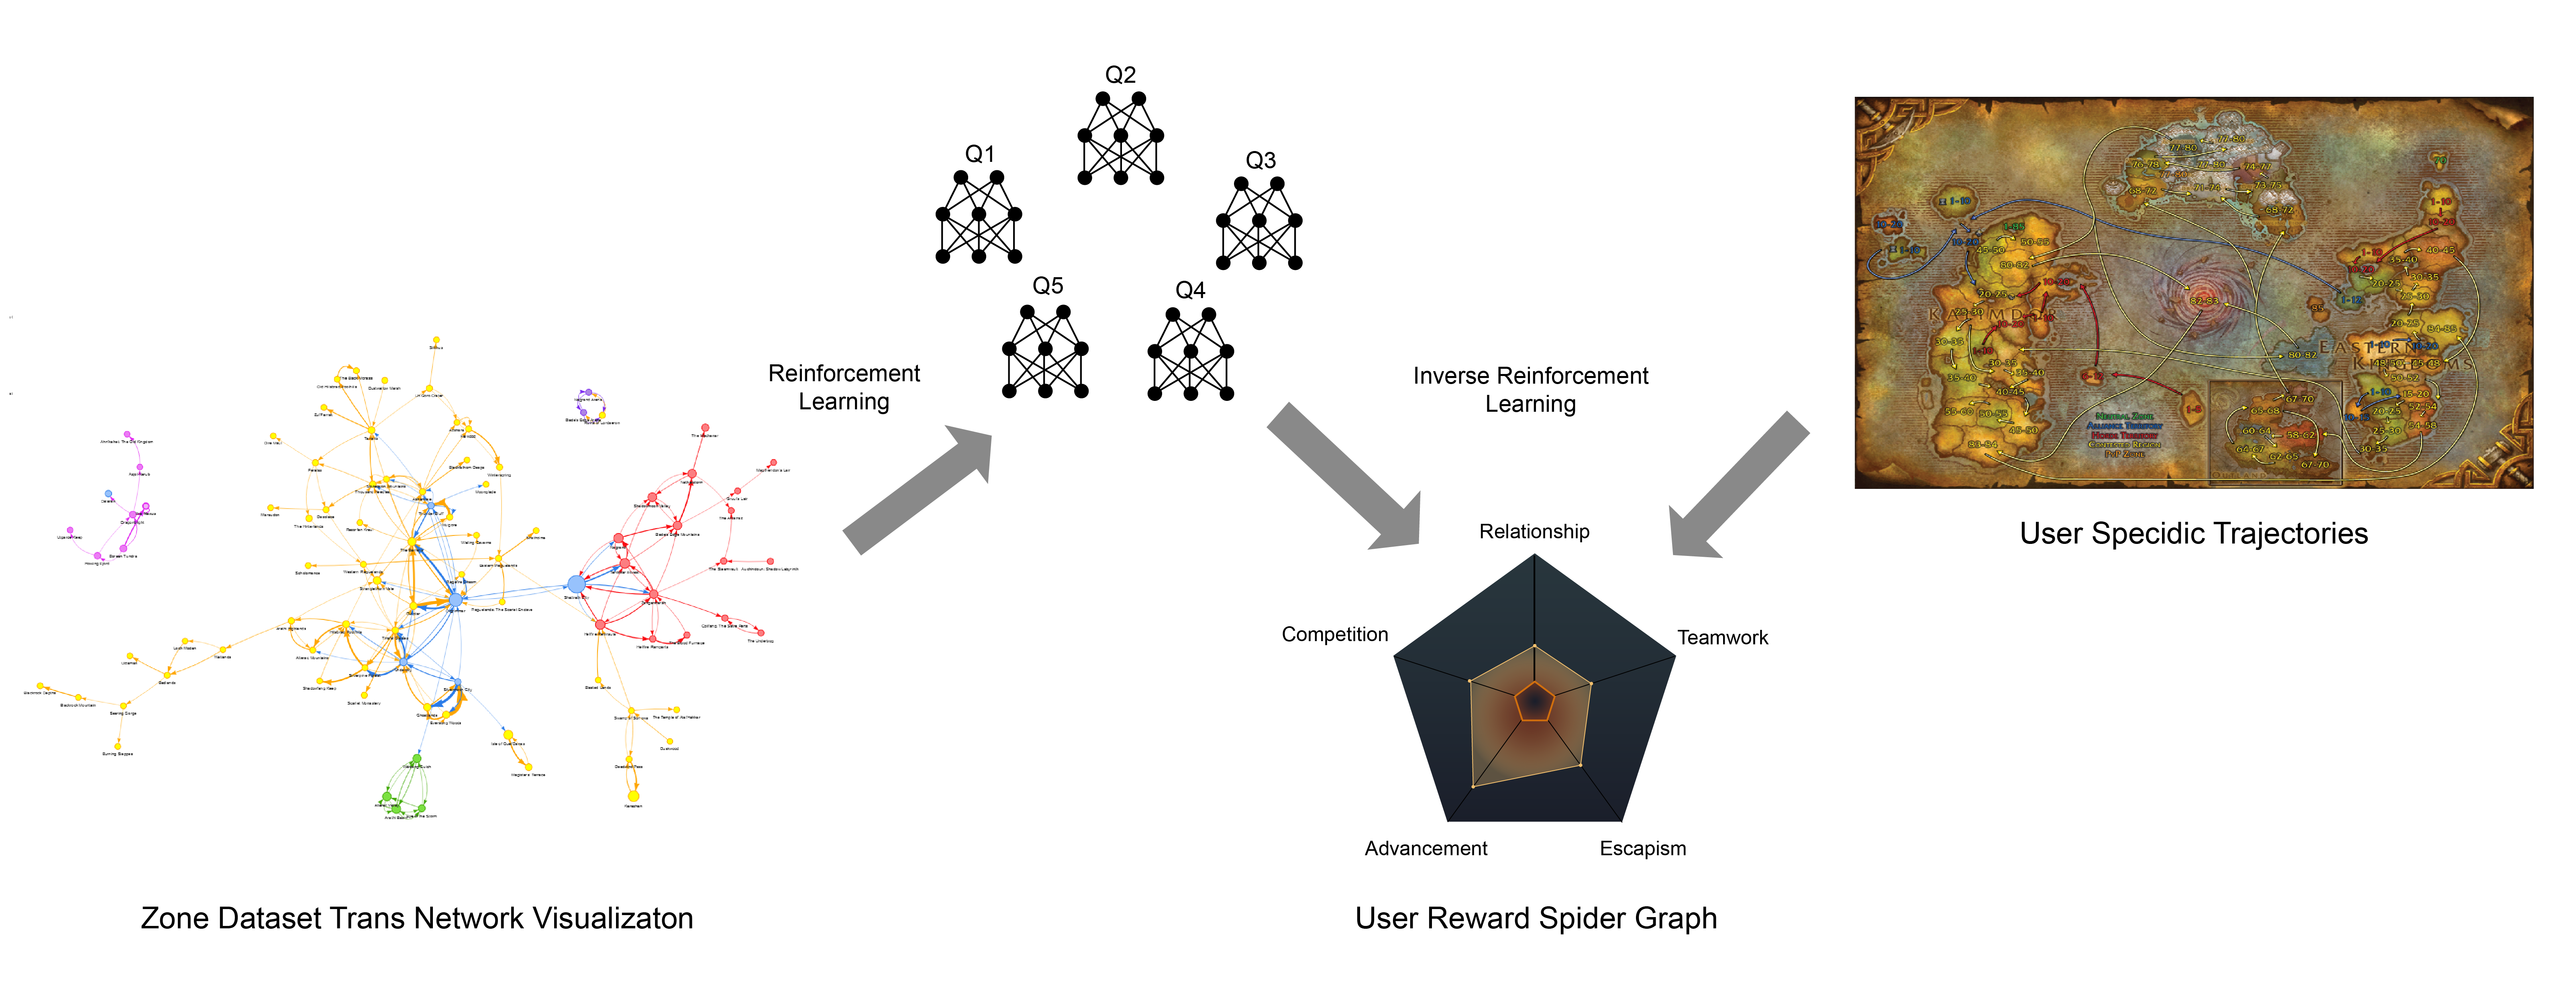
\includegraphics[width=\textwidth]{figs/workflow.png}
  \caption{Workflow to recovery the underlying reward mechanism using RL and IRL.}
  \label{fig:workflow}
\end{figure*}

\subsection{Action-Value Function Approximation}

To solve LP \eqref{eqn:lp} it suffices to estimate $Q^i(s,a)$. As the number of feasible states $s$ could be arbitrary large, for an user in WoW, it's impossible to enumerate over the state space. Instead, we use deep-Q networks (DQN) \cite{mnih2015human} to approximate the $Q^i$ functions. The neural network takes $s$ as input, and output the $Q$ value for every action $a$. We use the same network architecture for $i=1,\dots,5$, illustrated in Fig. \ref{fig:arch}. The categorical elements in $s$ are firstly processed by an embedding layer \cite{mikolov2013distributed}, while the numeral elements are fed into an fully connected (FC) layer with rectifier non-linearity. The output of embedding layer and FC layer are then concatenated and fed into another FC layer with rectifier nonlinearity. A final FC layer is applied to compute the $Q(s,a)$ value for each action $a$.

Denote the trainable parameters in the Q-network as $\theta^i$, we optimize over $\theta^i$ in order to approximate Eq. \eqref{eqn:qi}. The key observation of Q-learning is that, the action-value function, by its definition, should satisfy the Bellman equation. That is, if the user takes action $a$ and the state turns into $s_{t+1}$ from $s_t$, we have
\begin{equation}
Q^i(s_t,a_t)=r_{t} + \gamma \max_{a^\prime}Q^i(s_{t+1}, a^\prime). \label{eqn:bellman}
\end{equation}
Q-learning tries to find the action-value function satisfying Eq. \eqref{eqn:bellman}, by minimizing the squared difference $L$ between both sides of the equation. Let
\begin{equation*}
L^i=\mathbb{E}_{s_t, a_t, r_t, s_{t+1}} \frac{1}{2}(Q^i(s_t,a_t)- r_{t} - \gamma\max_{a^\prime}Q(s_{t+1}, a^\prime))^2.
\end{equation*}
Since $L^i$ is differentiable with respect to $\theta^i$, $\theta^i$ can be updated via stochastic gradient descent, by
\begin{eqnarray*}
\theta^i \leftarrow \theta^i - \alpha\frac{\partial L}{\partial \theta^i}\Big|_{s_t, a_t, r_t, s_{t+1}}
\end{eqnarray*}
We take advantage of the algorithm introduced in \cite{}, that the target network only get updated periodically, which is important for the stability of DQN training. The derivative of $L$ with respective $\theta^i$ becomes
$$\frac{\partial L}{\partial \theta^i} = \mathbb{E}\left[ (Q^i(s_t,a_t)- r_{t} + \gamma\max_{a^\prime}Q(s_{t+1}, a^\prime | \theta^{i -}))\cdot \frac{\partial{Q^i(s_t,a_t)}}{\partial{\theta^i}}\right],$$
where $\theta^{i-}$ is the network parameter which is assigned current $\theta^i$ value periodically during training.

\begin{figure*}[t]
  \centering
  \includegraphics[width=\textwidth]{figs/architecture.png}
  \caption{DQN architecture for $Q^i$ training, $i=1, \dots,5$}
  \label{fig:architecture}
\end{figure*}

\subsection{Policy and User Behaviors}

We conduct a quantitative evaluation of our learned $Q^1$ network. Consider collecting experience and getting level up is one of the major objective for players, we evaluate if the actions predicted by $Q^1$ agree with the moves conducted by those advancing players (who level up quickly). At state $s$, the predicted action is the one with the largest action-value $Q^1(s,a)$, i.e.,
\begin{equation*}
a = \text{argmax}_{a^\prime}Q^1(s,a^\prime).
\end{equation*}
For the $(s,a)$ pairs extracted from the top 200 (in leveling up speed) players' trajectories, the prediction accuracy is 0.49 with the total number of feasible actions $|\cup_s\mathcal{A}(s)|=156$, corresponding to 156 different zones in WoW existed during Jan 2006 - Jan 2009. It's competitive with 0.53, using policy cloning \cite{amit2002parametric,sammut1992learning} with classifier, and overperforms 0.23 if we approximate the $Q$ function using linear function. The quality of $Q^1$ is decent.

\section{Results}

Different from previous approaches on Atari games \cite{mnih2015human} and zero-sum games \cite{silver2016mastering,heinrich2016deep}, our approach models the user behavior instead of simply persuing advancement. Using Table. \ref{tbl:satisfactions} and solve LP \eqref{eqn:lp} on a dataset randomly drawn from the whole WoWAH dataset, the universal underlying reward mechanism of the player community is revealed as $\phi=(0.61, 0.16, 0.07, 0.05, 0.10)^T$. In another words, when conducting a behavior, in general the user's consideration is composed of 61\% there advancement, 16\% their competition, 7\% their relationship, 5\% their teamwork, and 10\% their escapism. The results is illustrated as a spider map in Fig. \ref{fig:spider}.

Armed with the model we conduct three different kinds further studies on WoWAH dataset. First we show that our model better describes the user behavior, than those who takes only single satisfaction metric. After recovering the underlying reward mechanism of the environment, our model could predict the move of the users, instead of just suggesting the best move for advancing (as $Q^1$ does). We then show the divergence of the underlying reward machenism between different groups of people, which is the causality driving the divergence of user behaviors. For example as the level of a player becomes higher, it tends to cares more about relationship than advancement. Finally we show, using our model, the evolution of underlying user satisfaction over time. Especially, observing the dynamics around the release of patch \textit{Fall of the Lich King}\footnote{http://wowwiki.wikia.com/wiki/Patch\_3.3.0}, it shed some light on quantitative models of the game design.

\begin{figure}[t]
    \centering
    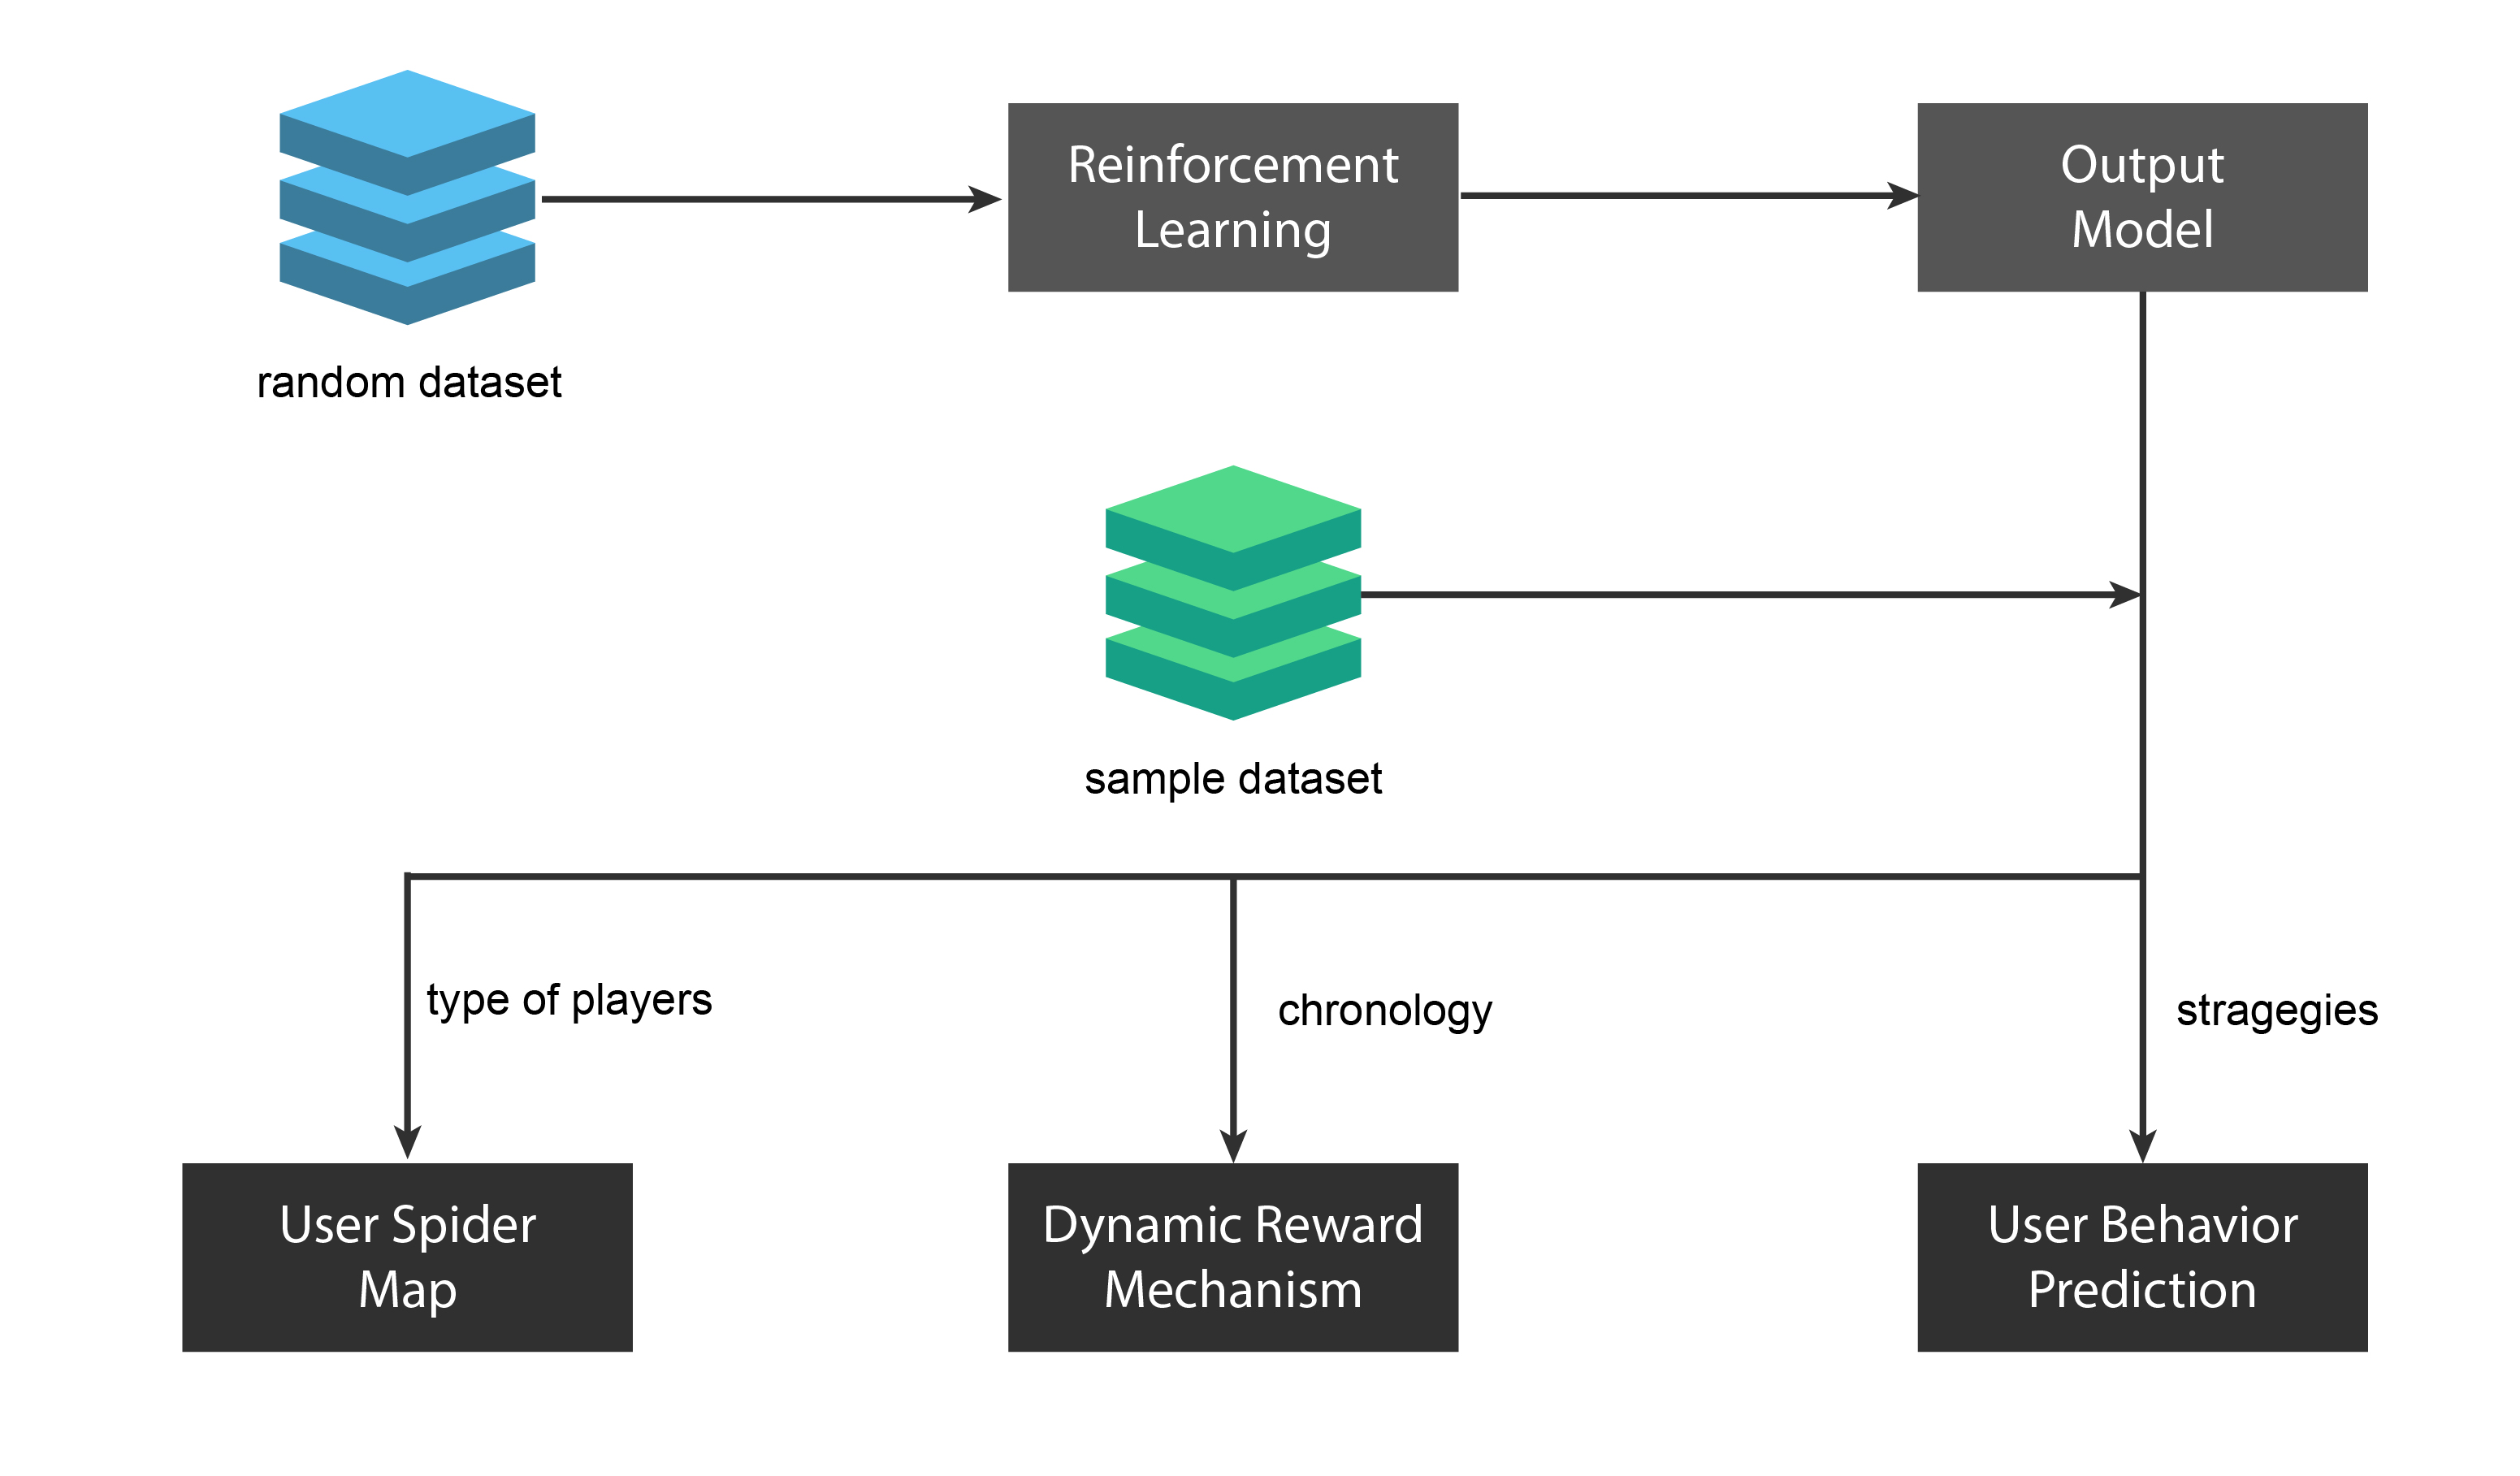
\includegraphics[width=\textwidth]{figs/results.jpg}
    \caption{Workflow to generate our results}
    \label{fig:results}
\end{figure}


\subsection{Predicting the Users' Behavior}

explain different game play styles

Armed with the reward mechanism we are able to model users' behavior instead of creating an agent to play the game itself. 
Consider that the users' motivation of playing is more than leveling up, 

Another interesting observation is the tradeoff between exploitation and exploration. In fact, many users' actions are sub-optimal, in the sense that they care too much about the satisfaction in the near future.

\subsection{Behavior Evolution over Time}

The way the user 

\subsection{Behavior Divergence between Different Groups of User}


\bibliographystyle{sigchi}
\bibliography{refs}

\end{document}
